\begin{frame}{Depósitos del Tesoro Nacional \small{(Fuente: Cálculos propios con base en MHCP)}} 
\begin{figure}
\centering
%\caption{Depósitos del Tesoro Nacional}
\label{fig:depositos}
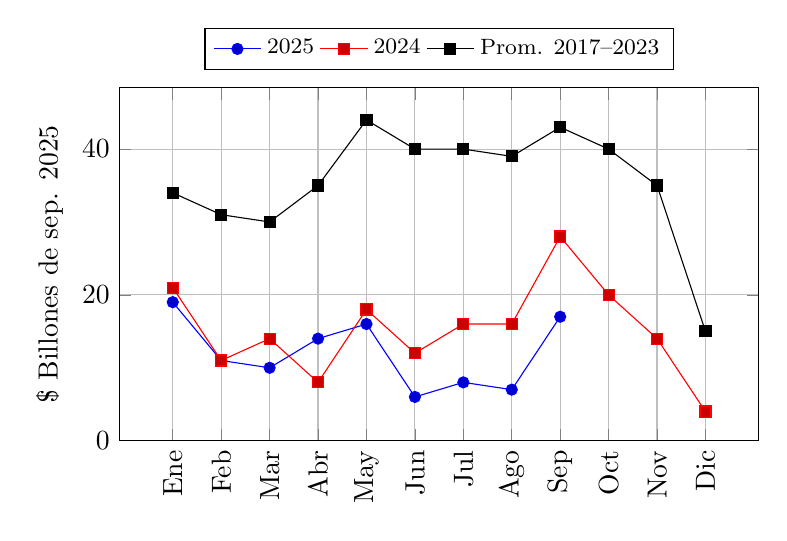
\begin{tikzpicture}
\begin{axis}[
    width=0.8\textwidth,
    height=0.5\textwidth,
    ylabel={ \$ Billones de sep. 2025},
    xtick={1,2,3,4,5,6,7,8,9,10,11,12},
    xticklabels={Ene,Feb,Mar,Abr,May,Jun,Jul,Ago,Sep,Oct,Nov,Dic},
    xticklabel style={rotate=90, anchor=east},
    legend columns=3,
    legend style={at={(0.5,1.05)},anchor=south},
    clip=false,
    grid=both,
    legend style={font=\footnotesize},
    ymin=0
]

% Valores de 2025
\addplot coordinates {
    (1,19) (2,11) (3,10) (4,14) (5,16) (6,6) 
    (7,8) (8,7) (9,17) 
};
\addlegendentry{2025}


% Valores de 2024
\addplot coordinates {
    (1,21) (2,11) (3,14) (4,8) (5,18) (6,12) 
    (7,16) (8,16) (9,28) (10,20) (11,14) (12,4)
};
\addlegendentry{2024}

% Prom 2017 a 2023
\addplot[mark=square*, color=black, solid] coordinates {
    (1,34) (2,31) (3,30) (4,35) (5,44) (6,40)
    (7,40) (8,39) (9,43) (10,40) (11,35) (12,15)
};
\addlegendentry{Prom. 2017--2023}

\end{axis}
\end{tikzpicture}
\vspace{0.1cm}
%\par\footnotesize{\textit{Fuente: Elaboración propia con base en datos de la Dirección de Crédito Público, Ministerio de Hacienda.}}
\end{figure}
\end{frame}
